\chapter{Theory}

Clearly the main problem in this project is obtaining the haemodynamic signal from the signal light intensity measured by the photodiodes. Or, rather, turning near infrared light into the measurement of brain activity.

\section{The Basics}

Analyzing the absorption spectra of light shows that the main absorbers in the near infrared light range (700nm - 900nm) are blood chromophores of oxyhaemoglobin (oxygenated haemoglobin, O$_{2}$Hb) and deoxyhaemoglobin (deoxygenated haemoglobin, HHb). Water and lipids absorb very little light, they are negligible and are basically transparent to near infrared light as depicted in Figure 3.1. Additionally it can be seen that in this spectral range, light is weakly absorbed by the tissue, making this spectral range ideal for NIRS imaging, which relies on reflected (backscattered) light. Thus, any changes in light intensity shone into the body can be interpreted as varying concentration levels of O$_{2}$Hb and HHb. These varying levels of oxygenation are used to estimate blood volume and tissue oxygenation, which indicate haemodynamic activity \cite{rosen05}.

\begin{figure}[htp]
\centering
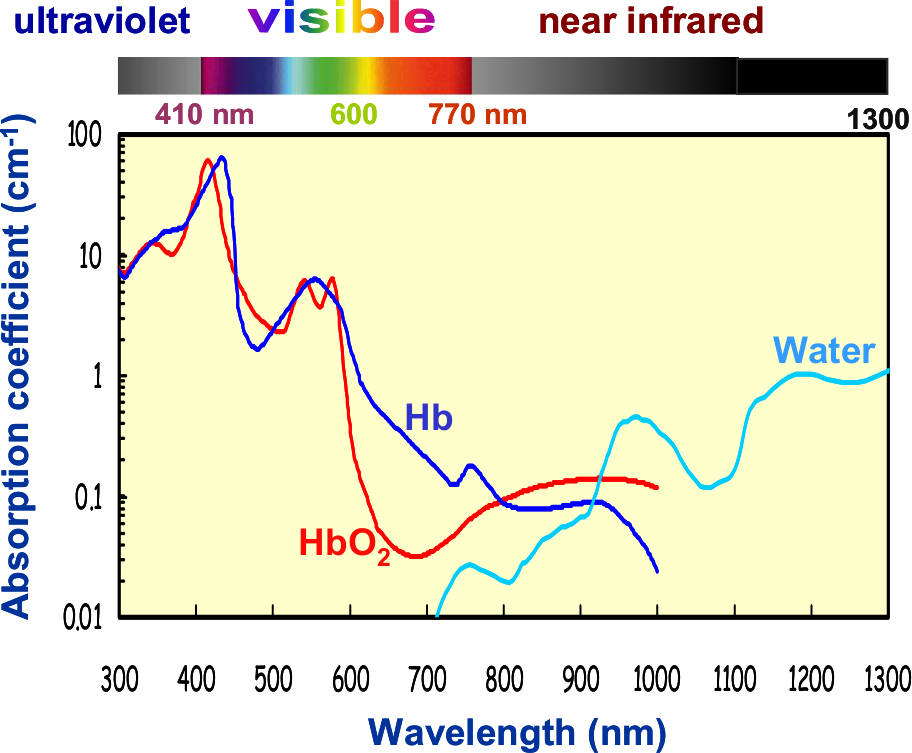
\includegraphics[width=4in]{spectra.png}
\caption[Propagation of photons]{Absorption spectra of deoxyhemoglobin (Hb), oxyhemoglobin (HbO$_2$), and water. The concentrations of Hb and HbO$_2$ are set to 50 μM$^1$.}
\end{figure}

\footnotetext[1]{Sergio Fantini’s Group, "Near-infrared spectroscopy for the study of biological tissue," Department of Biomedical Engineering, Tufts University, retrieved from http://ase.tufts.edu/biomedical/research/Fantini/researchAreas/NearInfraredSpectroscopy.pdf}

Near Infrared Light photons that are shone into the scalp are either absorbed by varying layers of tissue, such as the skin or the skull, scatter due to interactions with the tissue, or pass right through. Some of these scattered photons follow a kind of banana pattern through the head and back out due to the scattering effect of tissue (refer to figure 3.2). These backscattered photons can be picked up by a photodiode or a similar component \cite{rosen05}. However, now arises the problem of turning the measured light intensity into varying concentration levels of O$_{2}$Hb and HHb.

\begin{figure}[htp]
\centering
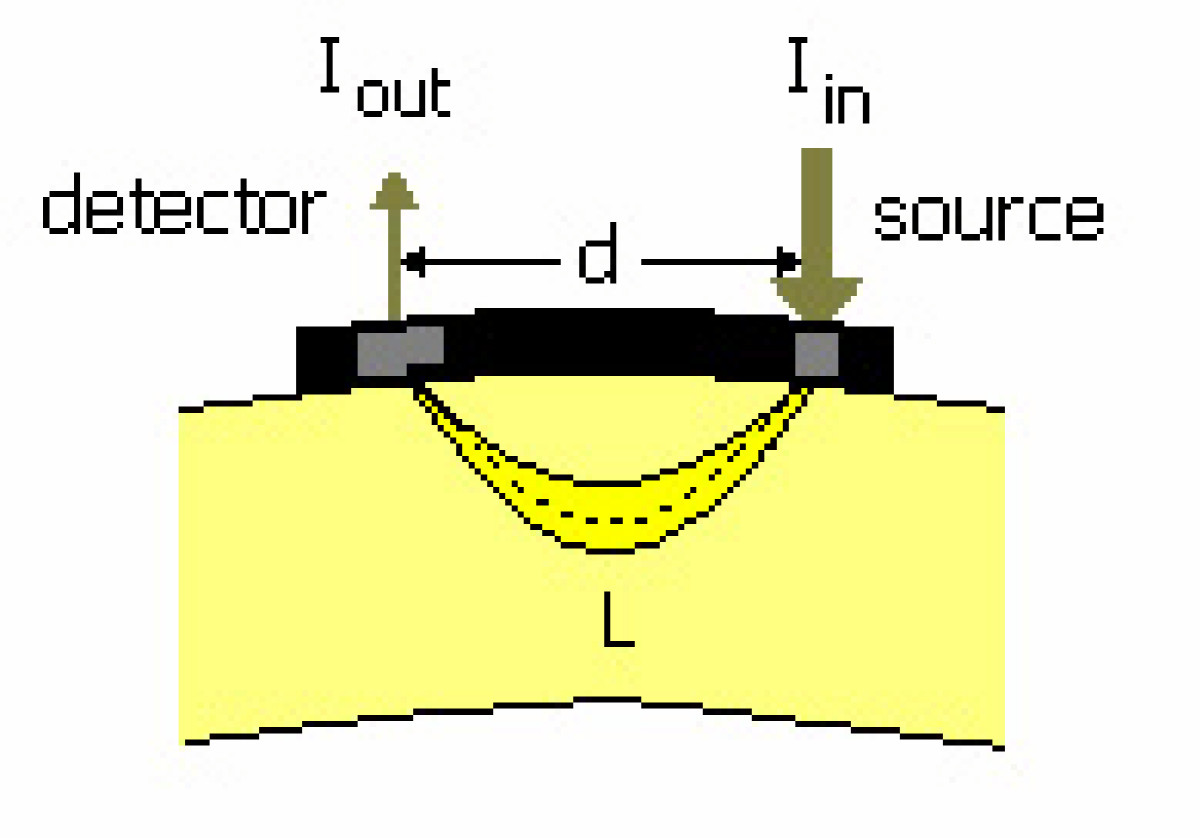
\includegraphics[width=4in]{banana.jpg}
\caption[Propagation of photons]{Propagation of photons from source to detector. The banana scattering pattern can clearly be seen here. \cite{rosen05}}
\end{figure}

\section {Modified Beer-Lambert Law}

This banana scattering effect is best described by the modified Beer-Lambert Law. The original Beer-Lambert law, A$^\lambda$ = $\epsilon^\lambda$cL, states the absorption of light (A) is proportional to the concentration of the absorber (c) multiplied by the specific wavelength extinction coefficient of the absorber ($\epsilon^\lambda$) and the path length the light has to travel (L, can be seen in Figure 3.2). However, this law only holds if the photons are absorbed or pass through the tissue in a straight line directly to the detector. Due to higher substance concentrations and substantial light scattering, the law does not hold in NIRS brain imaging \cite{chance97}. 

The modified law has to take into account the longer distance of light travel and loss of light intensity due to scattering. However, taking these into account would no longer purely calculate the amount of light absorbed. Rather it would find the amount of light absorbed and scattered or the total attenuation of the light, more accurately called optical density which varies for a different wavelength (OD$^\lambda$) \cite{rosen05}. Thus, introducing signal loss due to light scattering (G), the modified Beer-Lambert law becomes OD$^\lambda$ = $\epsilon^\lambda$cL + G. However, accurately measuring the path length of the light requires expensive highly specialized instruments. Thus, the pathlength the light has to travel can be estimated rather well by the distance between the light source and photodetector and the wavelength dependent differential pathlength factor (DPF$^\lambda$). That is,

\begin{equation}
L = d DPF^\lambda
\end{equation}
 
where d is the distance from the light source to the photodetector (refer to Figure 3.2) \cite{rosen05}. Assuming there is a constant light scattering loss, taking the average of two subsequent measurements the signal loss due to scattering (G) averages out. Producing the modified Beer-Lambert law this project is based on \cite{chance97}.

\begin{equation}
\Delta OD = \epsilon^\lambda c d\ DPF^\lambda
\end{equation}

Given the modified Beer-Lambert law, the light intensity measured by the photodiode in NIRS can accurately be described by 

\begin{equation}
I = I_{emitted} e^{-OD^\lambda}
\end{equation}

where I$_{emitted}$ is the light emitted by the light source into the head \cite{wolf05,rosen05}. Rearranging this equation gives

\begin{equation}
OD^\lambda = \ln \frac{I_{emitted}}{I}
\end{equation}

Taking the average of the optical density (or attenuation) between two subsequent measurements gives the equation

\begin{equation}
\Delta OD =  \ln \frac{I_{emitted}}{I_2} -  \ln \frac{I_{emitted}}{I_1} = \ln \frac{I_1}{I_2} = \epsilon^\lambda c d\ DPF^\lambda
\end{equation}

where I$_1$ is the first measurement and I$_2$ is the subsequent measurement \cite{yam02}. Since it is well documented that the main chromophores in blood that react to the near infrared light spectra are oxyhaemoglobin and deoxyhaemoglobin, finding the optical density in these cases is described by

\begin{equation}
\Delta OD = \ln \frac{I_1}{I_2} = (\epsilon^\lambda_{O_{2}Hb}\Delta c^\lambda_{O_{2}Hb} + \epsilon^\lambda_{HHb}\Delta c^\lambda_{HHb})  d\ DPF_\lambda
\end{equation}

where $\Delta$ c is the change in concentration of the specific chromosphore \cite{eke06}. Now if the attenuation of light (Optical Density) is measured at two different wavelengths $\lambda$1 and $\lambda$2, the above equation can be rearranged to yield

\begin{equation}
\Delta c_{O_{2}Hb}  =  \frac{\epsilon^{\lambda 1}_{HHb} \ \left (\frac{\displaystyle \Delta OD^{\lambda 2}}{\displaystyle d DPF^{\lambda 2}} \right) - \epsilon^{\lambda 2}_{HHb} \ \left (\displaystyle \frac{\Delta OD^{\lambda 1}}{\displaystyle d DPF^{\lambda 1}}\right)}{ \epsilon^{\lambda 1}_{HHb}\epsilon^{\lambda 2}_{O_{2}Hb} - \epsilon^{\lambda 2}_{HHb}\epsilon^{\lambda 1}_{O_{2}Hb}}
\end{equation}

\begin{equation}
\Delta c_{HHb}  =  \frac{\epsilon^{\lambda 1}_{O_{2}Hb} \ \left (\frac{\displaystyle \Delta OD^{\lambda 2}}{\displaystyle d DPF^{\lambda 2}}\right) - \epsilon^{\lambda 2}_{O_{2}Hb} 
\left (\frac{\displaystyle \Delta OD^{\lambda 1}}{\displaystyle d DPF^{\lambda 1}}\right)}{\epsilon^{\lambda 1}_{O_{2}Hb}\epsilon^{\lambda 2}_{HHb} - \epsilon^{\lambda 2}_{O_{2}Hb}\epsilon^{\lambda 1}_{HHb}}
\end{equation}

giving us the change in concentration between two measurements for oxyhaemoglobin and deoxyhaemoglobin \cite{eke06,yam02}. This can further be extended to find oxygenation of the blood and blood volume \cite{rosen05};

\begin{equation}
OXY = \Delta c_{O_{2}Hb} - \Delta c_{HHb}
\end{equation}

\begin{equation}
BV = \Delta c_{O_{2}Hb} + \Delta c_{HHb}
\end{equation}

It is important to note however the modified Beer-Lambert law used to derive the above equations is based on two assumptions: the absorption of the tissue changes homogeneously, and the light intensity lost due to scattering is constant. These assumptions are not true in practice. However, with appropriate wavelength selections for the light sources, these errors are minimal and negligible \cite{eke06}s.

It has been shown in past studies that brain activity as a result of a specific stimulation produces a highly localized increase in local oxygen consumption directly followed by an increase in blood flow within a few seconds, changing the O$_{2}$Hb and HHb concentrations \cite{freeman03}. Thus, we can conclude that changes in O$_{2}$Hb and HHb relate to brain activity.